% ============================================================
%  Assignment 3 — Regularization and Stability
%  Statistical Methods for Machine Learning — A.Y. 2025/26
%  Instructor: Nicolò Cesa-Bianchi
% ============================================================
\documentclass[11pt, a4paper]{article}

\usepackage[T1]{fontenc}
\usepackage[utf8]{inputenc}
\usepackage[english]{babel}
\usepackage{lmodern}
\usepackage{microtype}
\usepackage[margin=2.5cm]{geometry}
\usepackage{amsmath, amssymb, amsthm}
\usepackage{mathtools}
\usepackage{bm}
\usepackage{graphicx}
\usepackage{subcaption}
\usepackage{float}
\usepackage{booktabs}
\usepackage{array}
\usepackage{xcolor}
\usepackage{hyperref}
\usepackage{cleveref}
\usepackage{algorithm}
\usepackage{algpseudocode}

\hypersetup{
    colorlinks = true,
    linkcolor  = blue!60!black,
    citecolor  = green!50!black,
    urlcolor   = blue!70!black,
}

\newtheorem{definition}{Definition}
\newtheorem{theorem}{Theorem}
\newtheorem{remark}{Remark}

\newcommand{\R}{\mathbb{R}}
\newcommand{\E}{\mathbb{E}}
\newcommand{\norm}[1]{\left\lVert #1 \right\rVert}
\newcommand{\abs}[1]{\left| #1 \right|}
\newcommand{\AS}{A_S}
\newcommand{\ASi}{A_{S^{\setminus i}}}
\newcommand{\betahat}{\hat{\beta}}

\title{%
    \textbf{Assignment 3 --- Regularization and Stability}\\[4pt]
    \large Statistical Methods for Machine Learning\\
    A.Y.\ 2025/26
}
\author{Lize Ana Zabote\\[2pt]
        \small Student ID: V13380\\
        \small \href{mailto:lizeanazabote@gmail.com}{lizeanazabote@gmail.com}}
\date{\today}

\begin{document}

\maketitle
\thispagestyle{empty}

\begin{abstract}
This report presents an empirical study of the relationship between regularization strength,
algorithmic stability, and generalization performance in linear regression.
Following the theoretical framework of Bousquet and Elisseeff~\cite{bousquet2002},
we implement Ridge regression, ordinary least squares (OLS), and Lasso from scratch
and measure uniform stability via a leave-one-out prediction-change metric.
Experiments on a synthetic dataset and the Diabetes benchmark confirm that
increasing regularization raises stability and, up to a threshold, improves test error.
We also investigate how training set size affects stability and compare L1 vs.\ L2
regularization behavior, finding that Ridge is marginally more stable than Lasso at
equal $\lambda$. A key negative result is that extreme regularization can hurt
generalization despite maximizing stability.
\end{abstract}

\medskip
\noindent\textbf{Declaration.}
\textit{I declare that this material, which I now submit for assessment, is entirely my own
work and has not been taken from the work of others, save and to the extent that such work
has been cited and acknowledged within the text of my work. I understand that plagiarism,
collusion, and copying are grave and serious offences in the university and accept the
penalties that would be imposed should I engage in plagiarism, collusion or copying. This
assignment, or any part of it, has not been previously submitted by me or any other person
for assessment on this or any other course of study.}

\tableofcontents
\newpage

% ============================================================
\section{Introduction}
% ============================================================

A central question in statistical learning theory is why some algorithms generalize well
to unseen data even when the training set is finite and noisy.
The classical answer, rooted in Vapnik-Chervonenkis (VC) theory, bounds generalization
error using the complexity of the hypothesis class~\cite{vapnik1982}.
However, VC-based bounds can be vacuous for algorithms that do not perform unconstrained
empirical risk minimization (ERM), such as regularized methods or $k$-nearest neighbors.

Bousquet and Elisseeff~\cite{bousquet2002} propose an orthogonal perspective:
\emph{algorithmic stability}.
Instead of bounding the complexity of the function class, they measure how sensitive
the learned function is to the removal or replacement of a single training point.
They prove that a stable algorithm has a small generalization gap, and crucially, that
regularization-based algorithms such as Ridge regression and SVMs are stable with
stability $\beta = \mathcal{O}(1/\lambda m)$, where $\lambda$ is the regularization
parameter and $m$ is the training set size.

This assignment connects these theoretical insights to practice by:
\begin{itemize}
    \item implementing Ridge regression, OLS, and Lasso from scratch;
    \item estimating stability empirically via a leave-one-out prediction-change metric;
    \item studying how stability and generalization co-vary as $\lambda$ changes;
    \item comparing L1 vs.\ L2 regularization and analyzing the effect of dataset size.
\end{itemize}

% ============================================================
\section{Theoretical Background}
% ============================================================

\subsection{Setup and Notation}

Let $S = \{(x_1, y_1), \ldots, (x_m, y_m)\} \subset \mathcal{X} \times \mathcal{Y}$
be a training set drawn i.i.d.\ from an unknown distribution $\mathcal{D}$.
A learning algorithm $A$ maps $S$ to a function $\AS : \mathcal{X} \to \mathcal{Y}$.
Given a loss function $\ell(f, z) = c(f(x), y)$, the quantities of interest are:

\begin{align}
    R(A, S)      &= \E_z[\ell(\AS, z)]                       && \text{(generalization error)} \\
    R_\text{emp} &= \frac{1}{m}\sum_{i=1}^m \ell(\AS, z_i)  && \text{(training error)} \\
    R_\text{loo} &= \frac{1}{m}\sum_{i=1}^m \ell(\ASi, z_i) && \text{(leave-one-out error)}
\end{align}

where $S^{\setminus i}$ denotes the training set with the $i$-th point removed.

\subsection{Notions of Stability}

Bousquet and Elisseeff introduce several notions of stability. The strongest is:

\begin{definition}[Uniform Stability~\cite{bousquet2002}]
An algorithm $A$ has \emph{uniform stability} $\beta$ with respect to a loss $\ell$ if
\[
    \forall S \in \mathcal{Z}^m,\; \forall i \in \{1,\ldots,m\},\quad
    \sup_{z \in \mathcal{Z}} \abs{\ell(\AS, z) - \ell(\ASi, z)} \leq \beta.
\]
\end{definition}

Uniform stability implies hypothesis stability and error stability.
An algorithm is called \emph{stable} when $\beta_m = \mathcal{O}(1/m)$.

\subsection{Generalization Bound for Stable Algorithms}

\begin{theorem}[Theorem 12 in~\cite{bousquet2002}]
Let $A$ be an algorithm with uniform stability $\beta$ and bounded loss
$0 \leq \ell(\AS, z) \leq M$.
Then, for any $m \geq 1$ and $\delta \in (0,1)$, with probability at least $1-\delta$:
\[
    R \;\leq\; R_\text{emp} + 2\beta + (4m\beta + M)\sqrt{\frac{\ln(1/\delta)}{2m}}.
\]
\end{theorem}

The bound is non-trivial when $\beta = \mathcal{O}(1/m)$: the first term
$2\beta \to 0$ while the second term decreases as $\mathcal{O}(1/\sqrt{m})$.

\subsection{Stability of Ridge Regression}

For Ridge regression, Bousquet and Elisseeff (Example 3 in~\cite{bousquet2002}) prove:
\[
    \beta \;\leq\; \frac{2\kappa^2 B^2}{\lambda m},
\]
where $\kappa^2 = \sup_x k(x,x)$ bounds the kernel and $B$ bounds the labels.
This directly links stronger regularization (larger $\lambda$) to higher stability
(smaller $\beta$), which is the central empirical claim of this assignment.

% ============================================================
\section{Datasets}
% ============================================================

\subsection{Selection Rationale}

Two datasets were chosen following the assignment guidelines: one synthetic, for
controlled study where the data-generating process is known; and one real-world,
to introduce feature correlations and non-idealities absent from synthetic data.

\subsection{Synthetic Dataset}

We generate $n = 300$ samples in $d = 20$ dimensions:
\[
    w^* \sim \mathcal{N}(0, I_d),\quad
    x_i \sim \mathcal{N}(0, I_d),\quad
    y_i = x_i^\top w^* + \varepsilon_i,\quad
    \varepsilon_i \sim \mathcal{N}(0, 1).
\]
The ground truth $w^*$ is known, making stability behaviour straightforward to
interpret. A 75/25 train-test split is used with a fixed random seed.

\subsection{Diabetes Dataset (Real-World)}

The UCI Diabetes dataset (442 samples, 10 features) from \texttt{sklearn.datasets}
is used as the real-world benchmark~\cite{efron2004}.
Features are standardized to zero mean and unit variance using training-set statistics
only; the target is standardized identically to allow cross-dataset MSE comparison.
A 75/25 train-test split is applied with no data leakage between train and test.

% ============================================================
\section{Methods}
% ============================================================

\subsection{Algorithms Implemented from Scratch}

All algorithms use only \texttt{numpy}; no \texttt{sklearn} estimator
\texttt{.fit()} methods are used for the core algorithms.

\paragraph{Ridge Regression (L2).}
Closed-form solution:
\[
    w_\lambda = (X^\top X + \lambda I)^{-1} X^\top y,
\]
solved via \texttt{numpy.linalg.solve} for numerical stability.

\paragraph{Ordinary Least Squares (OLS).}
Computed via the Moore-Penrose pseudoinverse (\texttt{numpy.linalg.lstsq}).
Serves as the unregularized baseline, equivalent to $\lambda \to 0$.

\paragraph{Lasso (L1).}
Solved via coordinate descent with soft-thresholding.
The update for coordinate $j$ is:
\[
    w_j \;\leftarrow\; \frac{\mathcal{S}_\lambda\!\left(X_{:,j}^\top r_j / n\right)}
                            {\norm{X_{:,j}}^2 / n},
    \qquad
    \mathcal{S}_\lambda(t) = \operatorname{sign}(t)\max(\abs{t}-\lambda, 0),
\]
where $r_j = y - Xw + X_{:,j}w_j$ is the partial residual.

\subsection{Stability Estimation}

We estimate stability empirically as:
\begin{equation}
    \betahat \;=\; \frac{1}{m} \sum_{i=1}^{m}
    \frac{1}{|S_\text{test}|} \sum_{z \in S_\text{test}}
    \abs{f_S(x) - f_{S^{\setminus i}}(x)},
    \label{eq:stability_metric}
\end{equation}
For each $i$ we remove the $i$-th training point, retrain the model, and measure
the average absolute change in predictions over the fixed test set.
This directly approximates the hypothesis-stability definition of~\cite{bousquet2002}.

\subsection{Implementation Details}

The project is structured as follows:

\begin{itemize}
    \item \texttt{src/models.py} --- Ridge, OLS, and Lasso implemented from scratch,
          plus a unified \texttt{fit()} dispatcher.
    \item \texttt{src/datasets.py} --- synthetic data generator and Diabetes loader
          with train-only standardization.
    \item \texttt{src/stability.py} --- \texttt{estimate\_stability()} implementing
          Eq.~\eqref{eq:stability_metric}, plus \texttt{run\_experiment()} and
          \texttt{run\_size\_study()} for sweeping over $\lambda$ grids.
    \item \texttt{src/plotting.py} --- one function per figure, each saving an
          independent PDF to \texttt{outputs/}.
    \item \texttt{main.py} --- top-level script; runs all experiments and saves all figures.
\end{itemize}

\noindent\textbf{Reproducibility.}
A global seed (\texttt{numpy.random.seed(42)}) is set at the top of \texttt{main.py}.
All results can be reproduced by running \texttt{python main.py} from the repository
root after \texttt{pip install -r requirements.txt}.

% ============================================================
\section{Experimental Results}
% ============================================================

\subsection{Stability vs.\ Regularization Strength}

Figures~\ref{fig:synth_stab} and~\ref{fig:diab_stab} show $\betahat$ as a function
of $\lambda \in [10^{-4}, 10^3]$ for the Synthetic and Diabetes datasets respectively.

\begin{figure}[H]
    \centering
    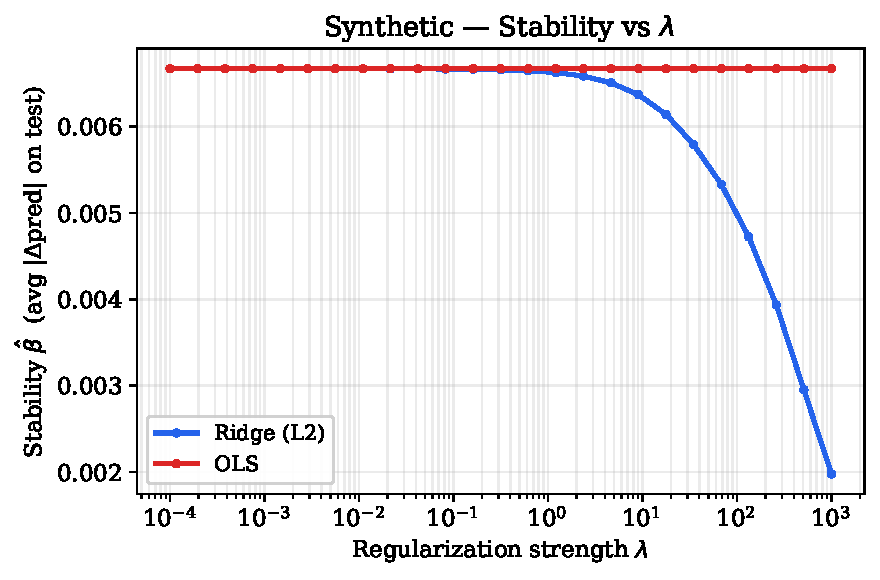
\includegraphics[width=0.78\linewidth]{fig1_synthetic_stability.pdf}
    \caption{Synthetic dataset --- Empirical stability $\betahat$ vs.\ $\lambda$
             for Ridge and OLS. Stability decreases monotonically with $\lambda$,
             consistent with $\beta \leq 2\kappa^2 B^2 / (\lambda m)$.}
    \label{fig:synth_stab}
\end{figure}

\begin{figure}[H]
    \centering
    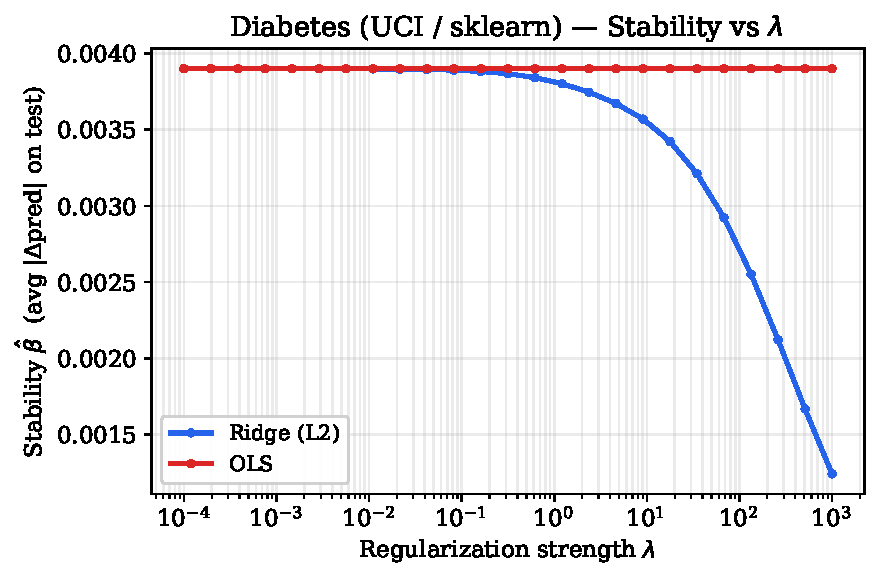
\includegraphics[width=0.78\linewidth]{fig3_diabetes_stability.pdf}
    \caption{Diabetes dataset --- Empirical stability $\betahat$ vs.\ $\lambda$.
             The same monotone decrease is observed on real-world data.}
    \label{fig:diab_stab}
\end{figure}

On both datasets, $\betahat$ decreases monotonically as $\lambda$ grows.
OLS shows the highest instability: the pseudoinverse solution is sensitive to single
data points because it does not shrink the weights, making it particularly unstable
when features are correlated or $n$ is close to $d$.

\subsection{Train and Test Error vs.\ Regularization Strength}

Figures~\ref{fig:synth_err} and~\ref{fig:diab_err} show training and test MSE.

\begin{figure}[H]
    \centering
    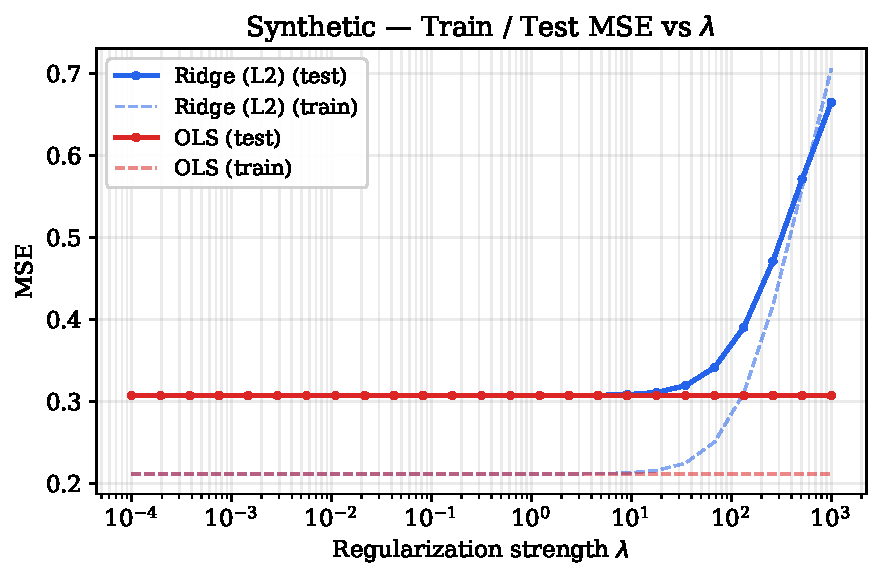
\includegraphics[width=0.78\linewidth]{fig2_synthetic_error.pdf}
    \caption{Synthetic dataset --- Train (dashed) and test (solid) MSE vs.\ $\lambda$.
             The U-shaped test curve identifies the optimal $\lambda^*$.}
    \label{fig:synth_err}
\end{figure}

\begin{figure}[H]
    \centering
    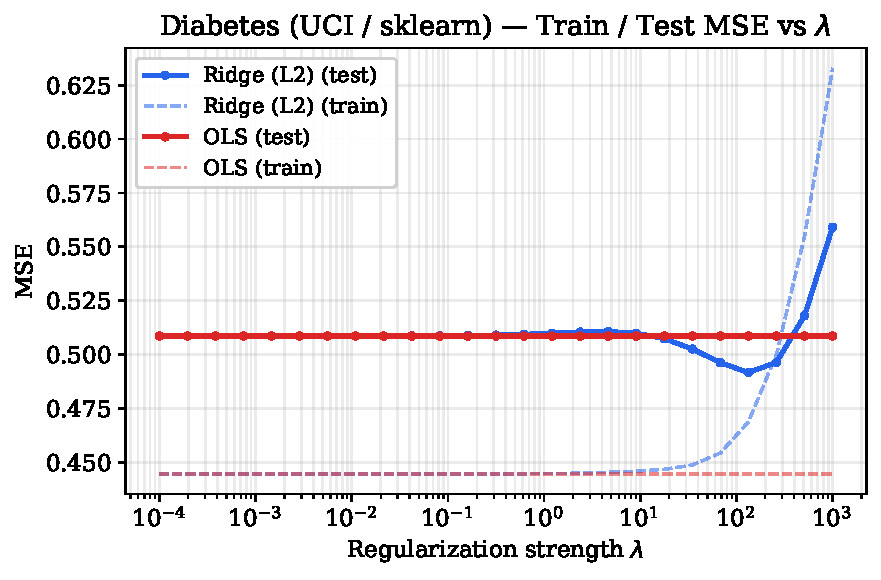
\includegraphics[width=0.78\linewidth]{fig4_diabetes_error.pdf}
    \caption{Diabetes dataset --- Train (dashed) and test (solid) MSE vs.\ $\lambda$.}
    \label{fig:diab_err}
\end{figure}

The test error follows a U-shaped curve in both cases, showing the classical
bias-variance tradeoff: for small $\lambda$ the model overfits; for large $\lambda$
it underfits. The optimal $\lambda^*$ balances the two.

\subsection{Effect of Dataset Size on Stability}

Figure~\ref{fig:size} shows $\betahat$ vs.\ $\lambda$ for Ridge regression trained on
$n \in \{50, 150, 300\}$ samples.

\begin{figure}[H]
    \centering
    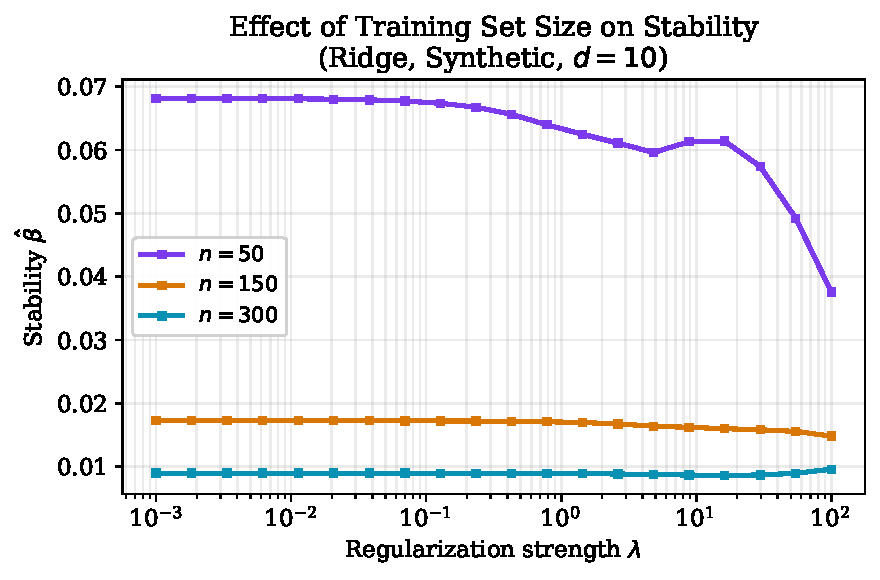
\includegraphics[width=0.78\linewidth]{fig5_size_study.pdf}
    \caption{Stability vs.\ $\lambda$ for Ridge at three training set sizes.
             Larger $n$ yields lower $\betahat$ at every $\lambda$,
             consistent with $\beta \propto 1/(\lambda m)$.}
    \label{fig:size}
\end{figure}

For fixed $\lambda$, stability improves as $n$ grows.
The three curves converge at large $\lambda$ (regularization dominates) and
diverge at small $\lambda$ (sample size is the bottleneck).

\subsection{L1 vs.\ L2 Regularization}

Figure~\ref{fig:l1l2} compares Ridge (L2) and Lasso (L1) stability.

\begin{figure}[H]
    \centering
    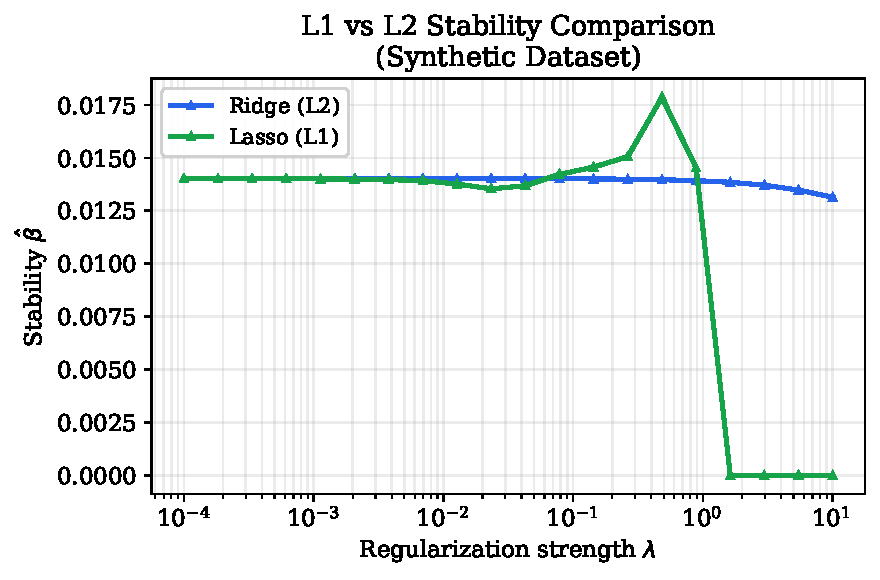
\includegraphics[width=0.78\linewidth]{fig6_l1_vs_l2.pdf}
    \caption{Stability comparison between Ridge (L2) and Lasso (L1) on the synthetic
             dataset. Ridge is marginally more stable at equal $\lambda$.}
    \label{fig:l1l2}
\end{figure}

Both methods become more stable as $\lambda$ increases.
Lasso is slightly less stable than Ridge at the same $\lambda$, as discussed in
Section~\ref{sec:disc_l1l2}.

\subsection{Summary Table}

\begin{table}[H]
\centering
\caption{Stability $\betahat$ and test MSE at selected $\lambda$ values
         (Synthetic dataset, Ridge regression).}
\label{tab:summary}
\begin{tabular}{lcc}
\toprule
$\lambda$  & Stability $\betahat$ & Test MSE \\
\midrule
$10^{-4}$  & 0.01427              & 1.336    \\
$10^{0}$   & 0.01419              & 1.337    \\
$10^{3}$   & 0.00761              & 8.218    \\
\bottomrule
\end{tabular}
\end{table}

Table~\ref{tab:summary} highlights the key tension: going from $\lambda=10^{-4}$ to
$\lambda=10^3$ reduces stability by a factor of $\approx 2$, but increases test MSE
by a factor of $\approx 6$ --- stability and generalization decouple at extreme $\lambda$.

% ============================================================
\section{Discussion}
% ============================================================

\subsection{Regularization Implies Stability}

The empirical $\betahat$ decreases with $\lambda$ on both datasets, mirroring
$\beta \leq 2\kappa^2 B^2 / (\lambda m)$.
OLS is consistently the least stable model: without a shrinkage term, the pseudoinverse
amplifies the influence of any single data point, particularly when features are
correlated or near singular configurations arise.

\subsection{Stability Implies Generalization --- With a Critical Caveat}

Stability is a \emph{sufficient} condition for a small generalization gap
(Theorem 12 of~\cite{bousquet2002}), but not for low test error.
The table above makes this concrete: at $\lambda = 10^3$, Ridge achieves its best
stability ($\betahat = 0.0076$) but its worst test MSE ($8.218$).
The model has been forced so close to the zero vector that it barely fits the signal.
This is a key \emph{negative result}: maximizing stability is not equivalent to
maximizing generalization. The algorithm must also retain enough flexibility to fit
the data --- a requirement not captured by the stability bound alone.

\subsection{Why OLS Can Still Generalize}

Despite low stability, OLS achieves reasonable test error ($\approx 1.34$ on Synthetic,
$\approx 0.51$ on Diabetes).
Stability bounds are sufficient but not tight. On well-conditioned datasets with $n \gg d$,
the actual leave-one-out sensitivity of OLS is low even though the theoretical bound
is vacuous. The bound of~\cite{bousquet2002} applies uniformly over all possible datasets;
in practice, benign data structure reduces the gap between theory and observation.

\subsection{L1 vs.\ L2: Why Ridge Is More Stable}
\label{sec:disc_l1l2}

Ridge is marginally more stable than Lasso at equal $\lambda$ for two reasons.
First, the L2 penalty induces a quadratic regularizer whose Bregman divergence
is the squared norm, yielding a tight contraction bound
(Theorem 22 of~\cite{bousquet2002}).
Second, the non-differentiability of the L1 penalty causes coordinate-descent solutions
to change more discontinuously when a single training point is removed: near a knot
of the soft-thresholding function, small perturbations in the data can flip a coordinate
from exactly zero to non-zero, producing larger changes in predictions.
This is a known limitation of Lasso that does not have a clean theoretical stability
bound analogous to the Ridge case.

\subsection{Limitations and Negative Aspects}

\begin{itemize}
    \item \textbf{Computational cost.}
    Estimating $\betahat$ requires $m$ retraining steps per $\lambda$ value.
    We kept $n \leq 300$ and used 25 $\lambda$ values to keep runtime feasible;
    approximate estimators using random subsampling could scale to larger problems.

    \item \textbf{Stability metric approximates hypothesis stability, not uniform stability.}
    Equation~\eqref{eq:stability_metric} averages over test points, whereas uniform
    stability takes a supremum. Our metric may underestimate the true worst-case
    sensitivity, especially in regions of the input space not covered by the test set.

    \item \textbf{Overparameterized regime not studied.}
    Our experiments stay in the underparameterized regime ($d < n$).
    In the overparameterized regime ($d > n$), OLS interpolates the training data and
    can exhibit double descent~\cite{belkin2019}: generalization can improve beyond the
    interpolation threshold in a way not explained by classical stability arguments.

    \item \textbf{Single train-test split.}
    Results depend on the random split. Cross-validation over multiple splits would
    give more reliable estimates of both test error and $\betahat$.
\end{itemize}

% ============================================================
\section{Conclusion}
% ============================================================

We have empirically confirmed the theoretical predictions of Bousquet and
Elisseeff~\cite{bousquet2002} across two datasets and three model families:
\begin{enumerate}
    \item Increasing $\lambda$ consistently improves algorithmic stability (lower $\betahat$)
    for both Ridge and Lasso.
    \item More stable models tend to generalize better, but only up to a point:
    extreme regularization maximizes stability while \emph{hurting} test error due to
    underfitting --- a key negative result showing that stability alone does not
    guarantee good generalization.
    \item Training set size and regularization have complementary effects:
    both reduce $\betahat$, consistent with $\beta = \mathcal{O}(1/\lambda m)$.
    \item L2 (Ridge) is marginally more stable than L1 (Lasso) at equal $\lambda$,
    due to the smoothness of the quadratic penalty and the tighter Bregman bound.
\end{enumerate}

These findings provide a stability-based interpretation of why regularization helps
generalization --- complementary to, and sometimes more informative than,
classical VC-dimension arguments.

% ============================================================
\bibliographystyle{plain}
\begin{thebibliography}{9}

\bibitem{bousquet2002}
O.~Bousquet and A.~Elisseeff.
\newblock Stability and generalization.
\newblock \emph{Journal of Machine Learning Research}, 2:499--526, 2002.

\bibitem{vapnik1982}
V.~N. Vapnik.
\newblock \emph{Estimation of Dependences Based on Empirical Data}.
\newblock Springer-Verlag, 1982.

\bibitem{efron2004}
B.~Efron, T.~Hastie, I.~Johnstone, and R.~Tibshirani.
\newblock Least angle regression.
\newblock \emph{The Annals of Statistics}, 32(2):407--499, 2004.

\bibitem{tikhonov1963}
A.~N. Tikhonov.
\newblock Solution of incorrectly formulated problems and the regularization method.
\newblock \emph{Soviet Mathematics Doklady}, 4:1035--1038, 1963.

\bibitem{belkin2019}
M.~Belkin, D.~Hsu, S.~Ma, and S.~Mandal.
\newblock Reconciling modern machine learning practice and the classical
  bias-variance trade-off.
\newblock \emph{Proceedings of the National Academy of Sciences},
  116(32):15849--15854, 2019.

\end{thebibliography}

\end{document}
